
% \begin{center}
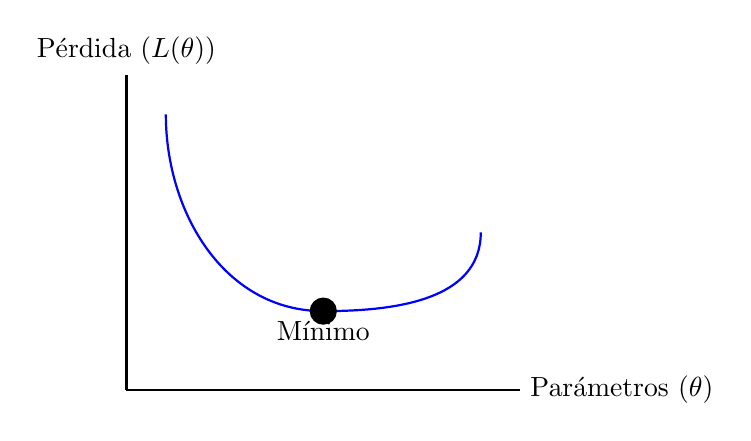
\begin{tikzpicture}[
        node distance=1.5cm,
        axis/.style={thick, -,'},
        loss/.style={rectangle, draw=red!50, fill=red!20, thick, minimum width=2cm, minimum height=1cm},
        dot/.style={circle, draw=black, fill=black, minimum size=0.1cm} % Definir estilo "dot"
    ]

    % Ejes
    \draw[axis] (0,0) -- (5,0) node[right] {Parámetros (\( \theta \))};
    \draw[axis] (0,0) -- (0,4) node[above] {Pérdida (\( L(\theta) \))};

    % Función de pérdida
    \draw[blue, thick] (0.5,3.5) to[out=270, in=180] (2.5,1) to[out=0, in=270] (4.5,2);

    % Punto mínimo
    \node[dot] at (2.5,1) {};
    \node[below] at (2.5,1) {Mínimo};

\end{tikzpicture}
% \end{center}
% \begin{tikzpicture}[very thick,radius=2cm]
%     \begin{scope}
%         \path[draw=black,fill=white] (0,0) circle;
%         \path[fill=red] (0,0) -- (2,0) arc [start angle=0, end angle=30];
%     \end{scope}
%     \begin{scope}[xshift=5cm]
%         \path[draw=black,fill=white] (0,0) circle;
%         \path[fill=red] (0,0) -- (2,0) arc [start angle=0, end angle=70];
%     \end{scope}
% \end{tikzpicture}